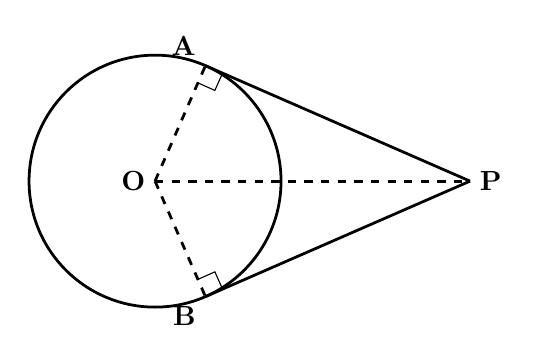
\begin{tikzpicture}[scale=0.8]
        % Circle centre and radius
        \coordinate (O) at (0,0);
        \draw[line width=1pt] (O) circle (2cm);
        
        % External point P
        \coordinate (P) at (5,0);
        
        % Tangent points A and B
        \coordinate (A) at (0.8, 1.833);
        \coordinate (B) at (0.8, -1.833);
        
        % Draw radius lines
        \draw[line width=1pt, dashed] (O) -- (A);
        \draw[line width=1pt, dashed] (O) -- (B);
        \draw[line width=1pt, dashed] (O) -- (P);
        
        % Draw tangent lines
        \draw[line width=1pt] (P) -- (A);
        \draw[line width=1pt] (P) -- (B);
        
        % Right angle indicators
        \draw (0.68, 1.56) -- (0.95, 1.44) -- (1.07, 1.71);
        \draw (0.68, -1.56) -- (0.95, -1.44) -- (1.07, -1.71);
        
        % Labels
        \node[left] at (O) {\textbf{O}};
        \node[right] at (P) {\textbf{P}};
        \node[above left] at (A) {\textbf{A}};
        \node[below left] at (B) {\textbf{B}};
    \end{tikzpicture}
